\documentclass[12pt, a4paper/letterpaper]{report}
\usepackage[margin=1in]{geometry}
\usepackage{graphicx, amsmath, enumitem}
\begin{document}
\begin{enumerate}[leftmargin=\labelsep]
\item
A marble rolls horizontally on a table top at a constant speed of 2.25 m/s. The marble rolls off the edge of the table and arcs towards the floor landing in a cup that is 1.50 m from the edge of the table. (No friction or air resistance). \\a) What is the height, $h$, of the table above the ground?\\b) What is the displacement $\vec{y}$ of the table top as measured from the top down to the ground

\vspace{10mm}

\item
A box slides across the floor from left to right with uniform (constant) acceleration. Starting from rest, it reaches a speed of 2.7 m/s in three seconds. \\ a) What is the acceleration, $\vec{a}$, of the box? \\ b) What is the displacement, $\vec{d}$, of the box after six seconds?

\vspace{10mm}

\item
The average distance between the sun and earth is defined to be the Astronomical Unit (AU): 1 AU = 1.50 $\times$ 10$^{11}$ m. Light (in the vacuum of space) moves at a constant speed of $c = 2.99 \times 10^8$ m/s. How long in minutes does it take light to reach the earth from the sun?

\vspace{10mm}

\item
What is the ideal banking angle $\theta$ for a gentle turn of radius 1.20 km on an interstate highway with a speed limit of 105 km/h (about 65 mi/h)?

\vspace{10mm}

\item
A toy dart gun uses a compressed spring to fire a dart of mass 0.100 kg horizontally. The spring in the toy has a spring constant $k = 250$ N/m and it is pushed in a distance of 6.0 cm from the relaxed position of the spring. \\ a) What $speed$ does the dart leave the barrel of the toy gun? (Hint: use conservation of energy). \\ b) If the toy is held horizontally above the ground at a height of 1.32 m when it is fired, how $far$ did the dart travel?

\vspace{10mm}

\item
A 5.0 kg rifle fires a 0.020 kg bullet from the barrel at 620 m/s. a) How $fast$ does the rifle recoil (move) backwards? b) If the rifle butt hits your shoulder and stops, how much kinetic energy (KE) is transformed?

\vspace{10mm}

\item
A centrifuge (a rotating device that separates mixtures) is accelerated from rest to 20,000 rpm (revolutions per minute) in 30 s. a) What is the $angular$ acceleration, $\alpha$. of the centrifuge? b) How many $degrees$, $\theta$, did the centrifuge rotate?

\vspace{10mm}

\item
A cylinder of mass $m = 1.32$ kg and radius $r = 0.25$ m rolls down a $25^{\circ}$ incline without slipping or friction. The incline is 1.25 m long. How $fast$ will it be moving at the bottom of the incline if it starts from rest at the top? The moment of inertia of a cylinder rotating about its axis is $I = (\frac{1}{2})mr^2$. \\ \begin{figure}[h] \begin{center} 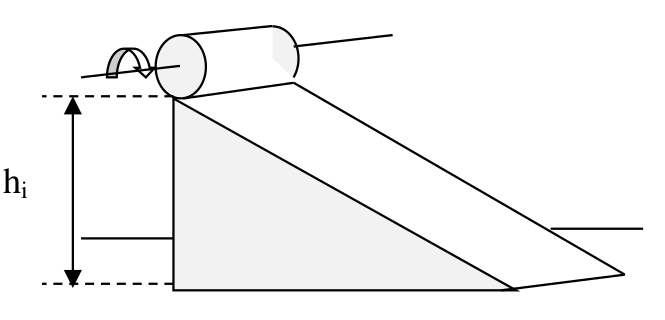
\includegraphics[scale=0.4]{pdb-14.png}\end{center} \end{figure}

\vspace{10mm}

\item
A bullet is fired from a rifle aimed horizontally (parallel to the ground) at the bullseye of a target. The speed at which the bullet leaves the barrel is 825 m/s. The bullet strikes 0.006 m directly below the bullseye. What horizontal distance did the bullet travel from the end of the rifle barrel to the target? Ignore air resistance.

\vspace{10mm}

\item
A 5.0 kg uniform horizontal beam 3.0 m in length is butted to a vertical wall and is supported by a wire that runs from the free end of the beam back to the wall at an angle of 36$^{\circ}$. What is the $tension$ $T$ in the wire if the beam is in equilibrium? \\  \begin{figure}[h] \begin{center} 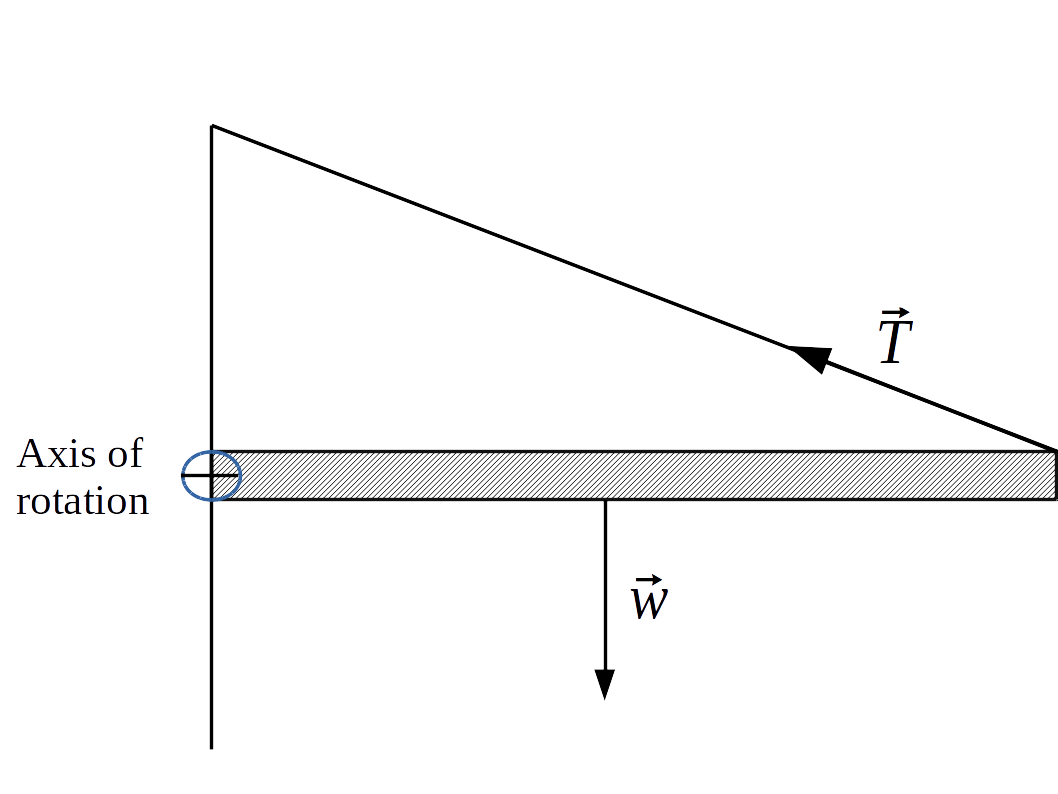
\includegraphics[scale=0.32] {pdb-25.png} \end{center} \end{figure}

\vspace{10mm}

\item
The take-up reel of a cassette tape has a radius of 0.015 m. Find the $length$ of tape that winds up around the reel in 5.3 s when the reel rotates at a uniform angular speed of 1.15 rad/s.

\vspace{10mm}

\item
A vector $\vec{A}$ of magnitude 3.45 km points at an angle of 48.5$^{\circ}$ from the x-axis. A second vector $\vec{B}$ of magnitude 2.44 km points at an angle of –19.3$^{\circ}$ from the x-axis. Find the vector sum of $\vec{A}+\vec{B}$ using vector components, giving the magnitude and direction of the sum.

\vspace{10mm}

\end{enumerate}
\end{document}
